\section{系统功能性需求分析}
\subsection{前台首页}

系统前台首页是平台最先展示给用户的页面,这里主要提供用户注册/登录入口、用户个人中心入口,实时展示影视舆情热点事件,并可更进一步查看某一事件的详情,以及平台的主要功能入口。平台提供的入口根据用户类别和功能需求可分为个人用户和企业用户,前者根据自身对影视舆情的兴趣浏览或搜索有关舆情事件或影视参与者及其相关信息系统,后者除了可以获取平台提供的舆情数据,还可以根据需求定制预警服务和分析报告等。前台首页的用例图如\textbf{图\ref{fig:fig1}} 所示,相关用例表如\textbf{表\ref{tab:tab1}}、\textbf{表\ref{tab:tab2}}、\textbf{表\ref{tab:tab3}}和\textbf{表\ref{tab:tab4}} 所示。

\begin{figure}[!htb]
	\centering\label{fig:fig1}
	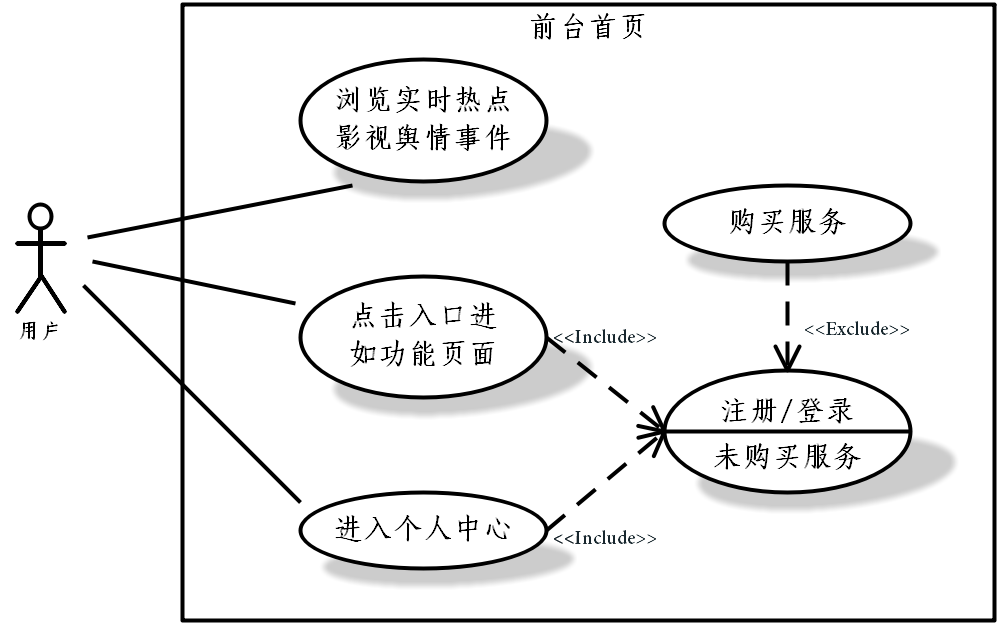
\includegraphics[scale=0.6]{image/f1.png}
	\caption{前台首页用例图}
\end{figure}



\begin{longtable}[c]{c|ccc}
	\caption{用户登录用例表}
	\label{tab:tab1}\\
	\shline
	\multicolumn{1}{c|}{\textbf{用例编号}} & \multicolumn{1}{c|}{UC-01} & \multicolumn{1}{c|}{用例名称} &  用户登录\\ \hline
	\endhead
	%
	\multicolumn{1}{c|}{\textbf{活动者}} & \multicolumn{1}{c|}{用户} & \multicolumn{1}{c|}{优先级} &高  \\ \hline
	\textbf{用例描述} & \multicolumn{3}{p{12cm}}{该用例用来描述用户打开平台首页页面后,状态为未登录的用户通过输入账号和密码进行登录操作,系统将在登录过程中对用户账号及密码的正确性进行验证,并判断用户为个人用户还是企业用户,在登录后根据不同的账号类型在部分页面进行不同的页面显示。} \\ \hline
	\textbf{前置条件}& \multicolumn{3}{p{12cm}}{用户通过浏览器输入平台地址。} \\ \hline
	\textbf{基本事件流}& \multicolumn{3}{p{12cm}}{用户打开浏览器,在地址栏输入平台网址;\newline
		打开平台,展示平台首页;\newline
		用户账号为未登录状态,点击登录;\newline
		展示登录页面;\newline
		输入用户账号和密码进行验证。} \\ \hline
	\textbf{异常事件流}& \multicolumn{3}{p{12cm}}{1.网址URL 输入错误,打开平台首页失败;\newline
		2.用户账号或密码错误,登录失败。
	} \\ \hline
	\textbf{后置条件}& \multicolumn{3}{p{12cm}}{页面由登录页面回到首页,用户登录状态为已登录。} \\ \shline
\end{longtable}

\begin{longtable}[c]{c|ccc}
	\caption{平台展示实时热点影视舆情事件用例表}
	\label{tab:tab2}\\
	\shline
	\multicolumn{1}{c|}{\textbf{用例编号}} & \multicolumn{1}{c|}{UC-02} & \multicolumn{1}{c|}{用例名称} &  实时展示热点舆情\\ \hline
	\endhead
	%
	\multicolumn{1}{c|}{\textbf{活动者}} & \multicolumn{1}{c|}{用户} & \multicolumn{1}{c|}{优先级} &高  \\ \hline
	\textbf{用例描述} & \multicolumn{3}{p{12cm}}{该用例用来描述用户打开平台首页页面后,即可浏览当前的热点影视舆情事件,想要深入了解的用户需要完成登录。} \\ \hline
	\textbf{前置条件}& \multicolumn{3}{p{12cm}}{用户通过浏览器输入平台地址。} \\ \hline
	\textbf{基本事件流}& \multicolumn{3}{p{12cm}}{用户打开浏览器,在地址栏输入平台网址;\newline
		打开平台,展示平台首页;\newline
		用户账号为未登录状态,可浏览简单的内容,想要深入了解,则展示登录页面;\newline
		输入用户账号和密码进行验证;\newline
		登录成功,可申请购买权限;\newline
		购买成功,可详细了解热点事件。} \\ \hline
	\textbf{异常事件流}& \multicolumn{3}{p{12cm}}{1.网址URL 输入错误,打开平台首页失败;\newline
	    2.用户账号或密码错误,登录失败;\newline
	    3.用户购买权限时出现支付异常等问题。
	} \\ \hline
	\textbf{后置条件}& \multicolumn{3}{p{12cm}}{页面由热点事件的详细内容页面回到首页。} \\ \shline
\end{longtable}

\begin{longtable}[c]{c|ccc}
	\caption{查看个人中心用例表}
	\label{tab:tab3}\\
	\shline
	\multicolumn{1}{c|}{\textbf{用例编号}} & \multicolumn{1}{c|}{UC-03} & \multicolumn{1}{c|}{用例名称} &  查看个人中心\\ \hline
	\endhead
	%
	\multicolumn{1}{c|}{\textbf{活动者}} & \multicolumn{1}{c|}{用户} & \multicolumn{1}{c|}{优先级} &中  \\ \hline
	\textbf{用例描述} & \multicolumn{3}{p{12cm}}{该用例用来描述用户完成登录后,根据用户的账号类型、个人信息和其他不同数据展示出不同的个人中心界面} \\ \hline
	\textbf{前置条件}& \multicolumn{3}{p{12cm}}{用户完成登录。} \\ \hline
	\textbf{基本事件流}& \multicolumn{3}{p{12cm}}{
		账号密码成功验证,用户完成登录;\newline
		用户点击个人中心按钮;\newline
		展示个人中心界面。
		} \\ \hline
	\textbf{异常事件流}& \multicolumn{3}{p{12cm}}{用户登录完成后未出现个人中心按钮。
	} \\ \hline
	\textbf{后置条件}& \multicolumn{3}{p{12cm}}{页面由个人中心界面返回首页,用户登录状态仍为已登录。} \\ \shline
\end{longtable}

\begin{longtable}[c]{c|ccc}
	\caption{点击功能入口用例表}
	\label{tab:tab4}\\
	\shline
	\multicolumn{1}{c|}{\textbf{用例编号}} & \multicolumn{1}{c|}{UC-04} & \multicolumn{1}{c|}{用例名称} &  功能入口\\ \hline
	\endhead
	%
	\multicolumn{1}{c|}{\textbf{活动者}} & \multicolumn{1}{c|}{用户} & \multicolumn{1}{c|}{优先级} &高  \\ \hline
	\textbf{用例描述} & \multicolumn{3}{p{12cm}}{该用例描述用户进入首页后,查看系统功能,若需使用各项功能需要用户完成登录并获取相应权限。} \\ \hline
	\textbf{前置条件}& \multicolumn{3}{p{12cm}}{用户成功打开首页。} \\ \hline
	\textbf{基本事件流}& \multicolumn{3}{p{12cm}}{用户点击功能入口查看系统功能;\newline
	    用户若想使用某项功能,需先登录;\newline
	    登陆成功,购买相应权限。
	} \\ \hline
	\textbf{异常事件流}& \multicolumn{3}{p{12cm}}{
		1.用户账号或密码错误,登录失败;\newline
		2.购买权限时支付出现异常。
	} \\ \hline
	\textbf{后置条件}& \multicolumn{3}{p{12cm}}{页面由功能页面跳转回首页。} \\ \shline
\end{longtable}

\subsection{个人中心}

个人中心模块需要展示用户个人账号基本信息,也可以查看一定事件段内的历史浏览记录和近期主要关注事件、人物等,并可查看相关数据。此外,还可以允许用户查看充值记录、系统消息等。企业用户还要能查看预警数据及详细说明和历史分析报告。用例图如\textbf{图\ref{fig:fig2}} 所示,相关用例表如\textbf{表\ref{tab:tab5}}、\textbf{表\ref{tab:tab6}}、\textbf{表\ref{tab:tab7}}、\textbf{表\ref{tab:tab8}}、\textbf{表\ref{tab:tab9}}和\textbf{表\ref{tab:tab10}}  所示。

\begin{figure}[!htb]
	\centering\label{fig:fig2}
	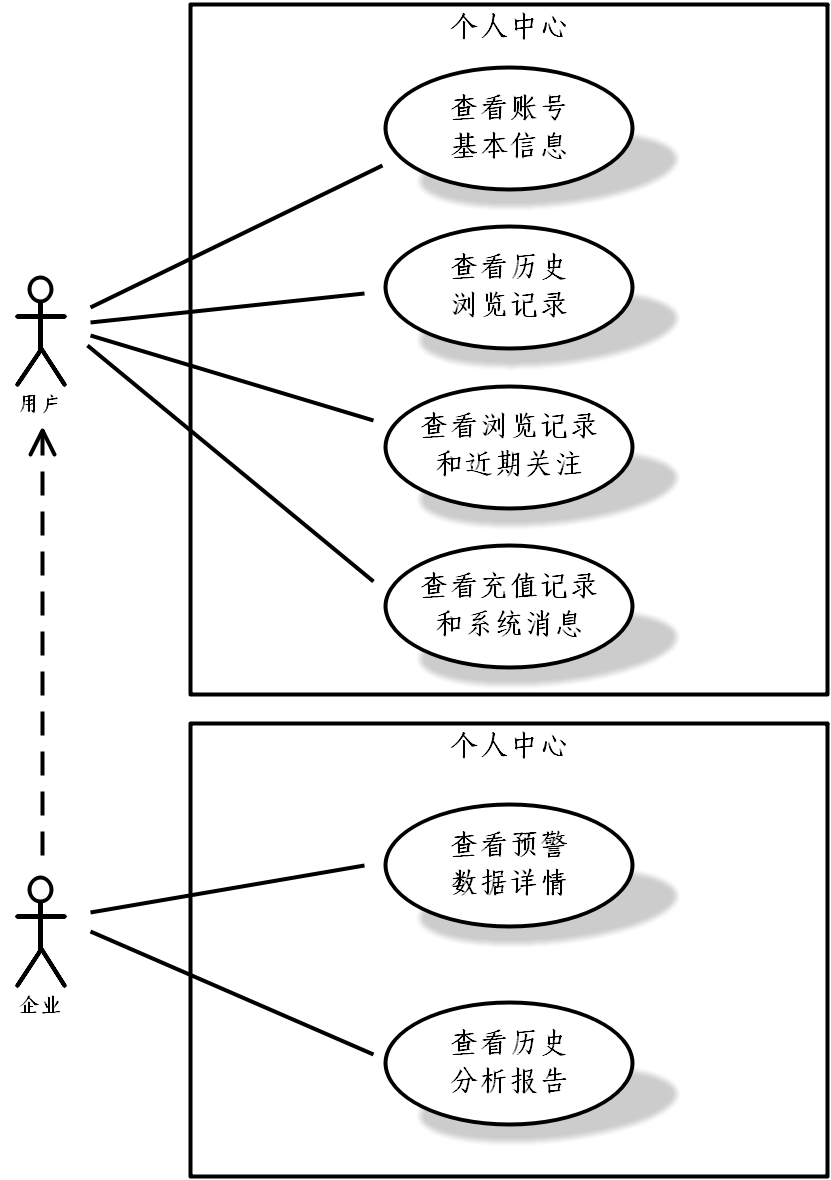
\includegraphics[scale=0.5]{image/f2.png}
	\caption{个人中心用例图}
\end{figure}

\begin{longtable}[c]{c|ccc}
	\caption{查看账号基本信息用例表}
	\label{tab:tab5}\\
	\shline
	\multicolumn{1}{c|}{\textbf{用例编号}} & \multicolumn{1}{c|}{UC-05} & \multicolumn{1}{c|}{用例名称} &  查看账号基本信息\\ \hline
	\endhead
	%
	\multicolumn{1}{c|}{\textbf{活动者}} & \multicolumn{1}{c|}{用户} & \multicolumn{1}{c|}{优先级} &低  \\ \hline
	\textbf{用例描述} & \multicolumn{3}{p{12cm}}{该用例用来描述用户进入个人中心界面后,查看自己的账号信息} \\ \hline
	\textbf{前置条件}& \multicolumn{3}{p{12cm}}{用户进入个人中心。} \\ \hline
	\textbf{基本事件流}& \multicolumn{3}{p{12cm}}{用户登录成功后,点击个人中心按钮进入个人中心界面;\newline
	    用户点击账号信息按钮,查看账号信息。
	} \\ \hline
	\textbf{异常事件流}& \multicolumn{3}{p{12cm}}{点击账号信息按钮,界面跳转出错。
	} \\ \hline
	\textbf{后置条件}& \multicolumn{3}{p{12cm}}{页面由账号信息界面返回个人中心界面。} \\ \shline
\end{longtable}

\begin{longtable}[c]{c|ccc}
	\caption{查看历史浏览数据用例表}
	\label{tab:tab6}\\
	\shline
	\multicolumn{1}{c|}{\textbf{用例编号}} & \multicolumn{1}{c|}{UC-06} & \multicolumn{1}{c|}{用例名称} &  查看历史浏览数据\\ \hline
	\endhead
	%
	\multicolumn{1}{c|}{\textbf{活动者}} & \multicolumn{1}{c|}{用户} & \multicolumn{1}{c|}{优先级} &中  \\ \hline
	\textbf{用例描述} & \multicolumn{3}{p{12cm}}{该用例用来描述用户进入个人中心界面,查看账号的历史浏览数据。} \\ \hline
	\textbf{前置条件}& \multicolumn{3}{p{12cm}}{用户进入个人中心。} \\ \hline
	\textbf{基本事件流}& \multicolumn{3}{p{12cm}}{用户登录成功后,点击个人中心按钮进入个人中心界面;\newline
	    用户点击浏览历史按钮,查看历史浏览数据。} \\ \hline
	\textbf{异常事件流}& \multicolumn{3}{p{12cm}}{点击历史浏览数据按钮,界面跳转异常。
	} \\ \hline
	\textbf{后置条件}& \multicolumn{3}{p{12cm}}{页面由历史浏览数据界面跳转回个人中心界面。} \\ \shline
\end{longtable}

\begin{longtable}[c]{c|ccc}
	\caption{查看近期关注用例表}
	\label{tab:tab7}\\
	\shline
	\multicolumn{1}{c|}{\textbf{用例编号}} & \multicolumn{1}{c|}{UC-07} & \multicolumn{1}{c|}{用例名称} &  查看近期关注\\ \hline
	\endhead
	%
	\multicolumn{1}{c|}{\textbf{活动者}} & \multicolumn{1}{c|}{用户} & \multicolumn{1}{c|}{优先级} &高  \\ \hline
	\textbf{用例描述} & \multicolumn{3}{p{12cm}}{该用例用来描述用户进入个人中心界面,点击近期关注按钮,查看该用户近期关注的热点事件或其他内容。} \\ \hline
	\textbf{前置条件}& \multicolumn{3}{p{12cm}}{用户进入个人中心。} \\ \hline
	\textbf{基本事件流}& \multicolumn{3}{p{12cm}}{用户登录成功后,点击个人中心按钮进入个人中心界面;\newline
	    用户点击近期关注按钮,查看历史浏览数据。} \\ \hline
	\textbf{异常事件流}& \multicolumn{3}{p{12cm}}{点击近期关注按钮,页面跳转异常。
	} \\ \hline
	\textbf{后置条件}& \multicolumn{3}{p{12cm}}{页面由近期关注界面跳转回个人中心界面。} \\ \shline
\end{longtable}

\begin{longtable}[c]{c|ccc}
	\caption{查看系统消息}
	\label{tab:tab8}\\
	\shline
	\multicolumn{1}{c|}{\textbf{用例编号}} & \multicolumn{1}{c|}{UC-08} & \multicolumn{1}{c|}{用例名称} &  查看系统消息\\ \hline
	\endhead
	%
	\multicolumn{1}{c|}{\textbf{活动者}} & \multicolumn{1}{c|}{用户} & \multicolumn{1}{c|}{优先级} &高  \\ \hline
	\textbf{用例描述} & \multicolumn{3}{p{12cm}}{该用例用来描述用户进入个人中心界面,点击系统消息按钮,查看该用户收到的系统消息。} \\ \hline
	\textbf{前置条件}& \multicolumn{3}{p{12cm}}{用户进入个人中心。} \\ \hline
	\textbf{基本事件流}& \multicolumn{3}{p{12cm}}{用户登录成功后,点击个人中心按钮进入个人中心界面;\newline
	    用户点击系统消息按钮,查看系统消息。} \\ \hline
	\textbf{异常事件流}& \multicolumn{3}{p{12cm}}{跳转系统消息页面时出错。
	} \\ \hline
	\textbf{后置条件}& \multicolumn{3}{p{12cm}}{页面由系统消息界面跳转回个人中心界面。} \\ \shline
\end{longtable}

\begin{longtable}[c]{c|ccc}
	\caption{查看历史分析报告用例表}
	\label{tab:tab9}\\
	\shline
	\multicolumn{1}{c|}{\textbf{用例编号}} & \multicolumn{1}{c|}{UC-09} & \multicolumn{1}{c|}{用例名称} &  查看历史分析报告\\ \hline
	\endhead
	%
	\multicolumn{1}{c|}{\textbf{活动者}} & \multicolumn{1}{c|}{用户} & \multicolumn{1}{c|}{优先级} &高  \\ \hline
	\textbf{用例描述} & \multicolumn{3}{p{12cm}}{该用例用来描述企业用户在进入个人中心界面后,查看历史分析报告。} \\ \hline
	\textbf{前置条件}& \multicolumn{3}{p{12cm}}{企业用户进入个人中心。} \\ \hline
	\textbf{基本事件流}& \multicolumn{3}{p{12cm}}{用户登录成功后,点击个人中心按钮进入个人中心界面;\newline
	    检查账户类型,企业用户显示历史分析报告按钮;\newline
	    用户点击历史分析报告按钮,查看历史分析报告。} \\ \hline
	\textbf{异常事件流}& \multicolumn{3}{p{12cm}}{1.账户类型判断异常;\newline
	    2.按钮显示异常;\newline
	    3.点击按钮后界面跳转异常。
	} \\ \hline
	\textbf{后置条件}& \multicolumn{3}{p{12cm}}{页面由历史分析报告页面回到个人中心界面。} \\ \shline
\end{longtable}

\begin{longtable}[c]{c|ccc}
	\caption{查看预警详情用例表}
	\label{tab:tab10}\\
	\shline
	\multicolumn{1}{c|}{\textbf{用例编号}} & \multicolumn{1}{c|}{UC-10} & \multicolumn{1}{c|}{用例名称} &  查看预警详情\\ \hline
	\endhead
	%
	\multicolumn{1}{c|}{\textbf{活动者}} & \multicolumn{1}{c|}{用户} & \multicolumn{1}{c|}{优先级} &高  \\ \hline
	\textbf{用例描述} & \multicolumn{3}{p{12cm}}{该用例用来描述企业用户在进入个人中心界面后,查看预警详情。} \\ \hline
	\textbf{前置条件}& \multicolumn{3}{p{12cm}}{企业用户进入个人中心。} \\ \hline
	\textbf{基本事件流}& \multicolumn{3}{p{12cm}}{用户登录成功后,点击个人中心按钮进入个人中心界面;\newline
	    检查账户类型,企业用户显示预警详情按钮;\newline
	    用户点击预警详情按钮,查看预警详情。} \\ \hline
	\textbf{异常事件流}& \multicolumn{3}{p{12cm}}{1.账户类型判断异常;\newline
	    2.按钮显示异常;\newline
	    3.点击按钮后界面跳转异常。
	} \\ \hline
	\textbf{后置条件}& \multicolumn{3}{p{12cm}}{页面由预警详情页面回到个人中心界面。} \\ \shline
\end{longtable}

\subsection{个人用户页面}
购买个人服务的用户,可以通过平台首页进入个人用户页面,而未获得此项服务的用户(或游客账号)在点击首页入口时,则会由于权限认证失败而收到邀请购买服务的询问。在进入个人用户页面后,用户可以通过平台提供的类别,如人物(导演、艺人、自媒体制作人等)和题材(电视剧、电影、综艺等)筛选热点舆情事件,也可以在搜索栏中通过关键词进行筛选。在点击相关词条后,可以进入舆情事件的详情界面。用户也可以根据喜好将关注的影视舆情事件参与者、影视剧作品等设为关注列表添加到该页面。用例图如\textbf{图\ref{fig:fig3}} 所示,相关用例表如\textbf{表\ref{tab:tab11}}和\textbf{表\ref{tab:tab12}} 所示。

\begin{figure}[!htb]
	\centering\label{fig:fig3}
	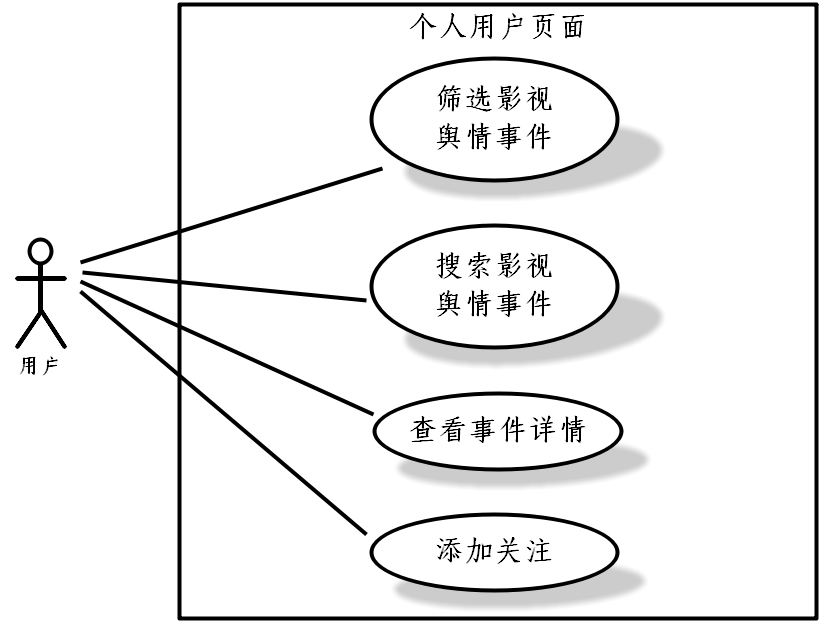
\includegraphics[scale=0.5]{image/f3.png}
	\caption{个人用户页面用例图}
\end{figure}

\begin{longtable}[c]{c|ccc}
	\caption{筛选影视舆情事件用例表}
	\label{tab:tab11}\\
	\shline
	\multicolumn{1}{c|}{\textbf{用例编号}} & \multicolumn{1}{c|}{UC-11} & \multicolumn{1}{c|}{用例名称} &  筛选影视舆情事件\\ \hline
	\endhead
	%
	\multicolumn{1}{c|}{\textbf{活动者}} & \multicolumn{1}{c|}{用户} & \multicolumn{1}{c|}{优先级} &高  \\ \hline
	\textbf{用例描述} & \multicolumn{3}{p{12cm}}{该用例用来描述用户进入个人用户页面后筛选影视舆情事件。} \\ \hline
	\textbf{前置条件}& \multicolumn{3}{p{12cm}}{用户进入个人用户页面。} \\ \hline
	\textbf{基本事件流}& \multicolumn{3}{p{12cm}}{用户进入个人用户页面;\newline
	    点击筛选/搜索按钮进行影视舆情事件的筛选或搜索。
	} \\ \hline
	\textbf{异常事件流}& \multicolumn{3}{p{12cm}}{
	    1.用户输入不明字符;\newline
	    2.页面跳转或搜索结果异常。
	} \\ \hline
	\textbf{后置条件}& \multicolumn{3}{p{12cm}}{用户由筛选结果页面跳转至个人用户界面。} \\ \shline
\end{longtable}

\begin{longtable}[c]{c|ccc}
	\caption{添加关注用例表}
	\label{tab:tab12}\\
	\shline
	\multicolumn{1}{c|}{\textbf{用例编号}} & \multicolumn{1}{c|}{UC-12} & \multicolumn{1}{c|}{用例名称} &  添加关注\\ \hline
	\endhead
	%
	\multicolumn{1}{c|}{\textbf{活动者}} & \multicolumn{1}{c|}{用户} & \multicolumn{1}{c|}{优先级} &中  \\ \hline
	\textbf{用例描述} & \multicolumn{3}{p{12cm}}{该用例用来描述用户进入个人用户界面后,添加关注。} \\ \hline
	\textbf{前置条件}& \multicolumn{3}{p{12cm}}{用户进入个人用户界面。} \\ \hline
	\textbf{基本事件流}& \multicolumn{3}{p{12cm}}{用户进入个人用户界面;\newline
	    用户进入关注页面,对想要关注的内容添加关注。
	} \\ \hline
	\textbf{异常事件流}& \multicolumn{3}{p{12cm}}{
	    1.界面跳转异常;\newline
	    2.数据记录未实时更新。
	} \\ \hline
	\textbf{后置条件}& \multicolumn{3}{p{12cm}}{页面由关注页面回到个人用户页面。} \\ \shline
\end{longtable}

\subsection{企业用户页面}
购买企业服务的用户,可以通过平台首页进入企业用户页面,而未获得此项服务的用户(如游客账号或个人用户账号)在点击首页入口时,则会由于权限认证失败而收到邀请进行企业认证并购买服务的询问。在进入企业用户页面后,用户可以通过平台提供的类别,如人物(导演、艺人、自媒体制作人等)和题材(电视剧、电影、综艺等)筛选热点舆情事件,也可以在搜索栏中通过关键词进行筛选。在点击相关词条后,可以进入舆情事件的详情界面。用户也可以定制某一舆情事件或影视及相关人员的舆情预警、期末查看本月(或年)的舆情数据分析报告,并可以定制营销效果分析。用例图如\textbf{图\ref{fig:fig4}} 所示,相关用例表如\textbf{表\ref{tab:tab13}} 所示。

\begin{figure}[!htb]
	\centering\label{fig:fig4}
	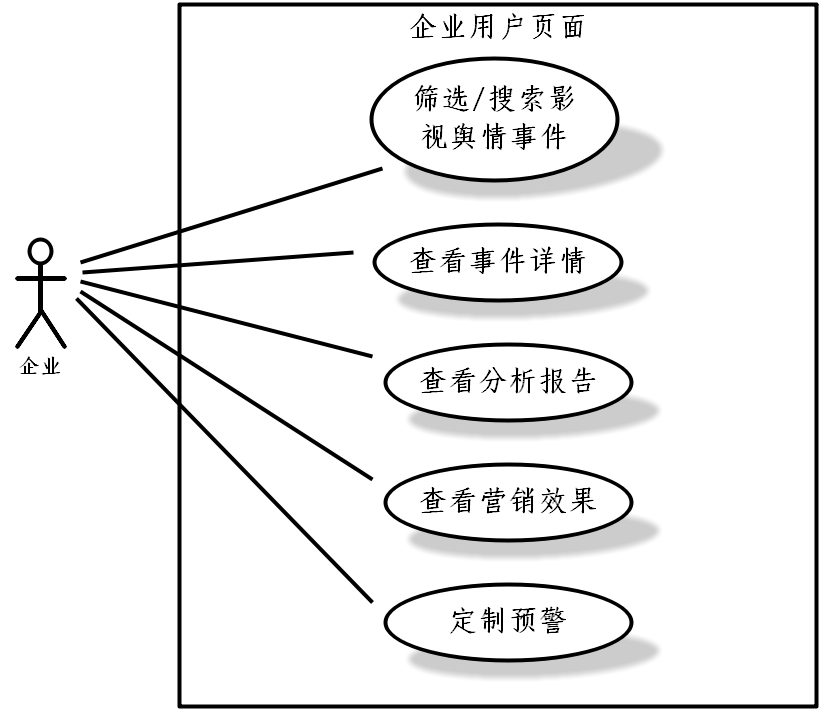
\includegraphics[scale=0.5]{image/f4.png}
	\caption{企业用户页面用例图}
\end{figure}

\begin{longtable}[c]{c|ccc}
	\caption{查看分析数据用例表}
	\label{tab:tab13}\\
	\shline
	\multicolumn{1}{c|}{\textbf{用例编号}} & \multicolumn{1}{c|}{UC-13} & \multicolumn{1}{c|}{用例名称} &  查看分析数据\\ \hline
	\endhead
	%
	\multicolumn{1}{c|}{\textbf{活动者}} & \multicolumn{1}{c|}{用户} & \multicolumn{1}{c|}{优先级} &高  \\ \hline
	\textbf{用例描述} & \multicolumn{3}{p{12cm}}{该用例用来描述企业用户进入企业用户界面后,查看分析数据。} \\ \hline
	\textbf{前置条件}& \multicolumn{3}{p{12cm}}{用户进入企业用户界面。} \\ \hline
	\textbf{基本事件流}& \multicolumn{3}{p{12cm}}{用户进入企业用户界面;\newline
	    用户点击分析数据按钮,查看分析数据。
	} \\ \hline
	\textbf{异常事件流}& \multicolumn{3}{p{12cm}}{页面跳转出错。
	} \\ \hline
	\textbf{后置条件}& \multicolumn{3}{p{12cm}}{页面由数据分析页面回到企业用户页面。} \\ \shline
\end{longtable}

\subsection{舆情事件详情页面}
购买平台服务的用户,在通过系统认证后,可以通过不同的功能入口进行影视舆情事筛选,并经由筛选出的词条进入详情界面查看影视参与者或影视作品的有关信息,例如事件的主要人物、人物关系图谱、事件时间轴、事件情感分析与关注度等,通过关系图谱和时间轴的结点可以查看相关信息。用例图如\textbf{图\ref{fig:fig5}} 所示,相关用例表如\textbf{表\ref{tab:tab14}} 所示。

\begin{figure}[!htb]
	\centering\label{fig:fig5}
	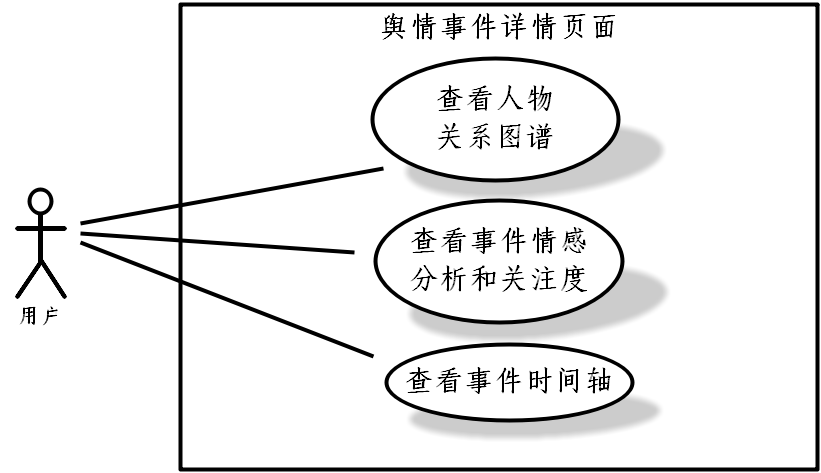
\includegraphics[scale=0.5]{image/f5.png}
	\caption{舆情事件详情页面用例图}
\end{figure}

\begin{longtable}[c]{c|ccc}
	\caption{查看舆情事件详情用例表}
	\label{tab:tab14}\\
	\shline
	\multicolumn{1}{c|}{\textbf{用例编号}} & \multicolumn{1}{c|}{UC-01} & \multicolumn{1}{c|}{用例名称} &  用户登录\\ \hline
	\endhead
	%
	\multicolumn{1}{c|}{\textbf{活动者}} & \multicolumn{1}{c|}{用户} & \multicolumn{1}{c|}{优先级} &高  \\ \hline
	\textbf{用例描述} & \multicolumn{3}{p{12cm}}{该用例用来描述用户打开平台首页页面后,状态为未登录的用户通过输入账号和密码进行登录操作,系统将在登录过程中对用户账号及密码的正确性进行验证,并判断用户为个人用户还是企业用户,在登录后根据不同的账号类型在部分页面进行不同的页面显示。} \\ \hline
	\textbf{前置条件}& \multicolumn{3}{p{12cm}}{用户通过浏览器输入平台地址。} \\ \hline
	\textbf{基本事件流}& \multicolumn{3}{p{12cm}}{用户打开浏览器,在地址栏输入平台网址;\newline
		打开平台,展示平台首页;\newline
		用户账号为未登录状态,点击登录;\newline
		展示登录页面;\newline
		输入用户账号和密码进行验证。} \\ \hline
	\textbf{异常事件流}& \multicolumn{3}{p{12cm}}{1.网址URL 输入错误,打开平台首页失败;\newline
		2.用户账号或密码错误,登录失败。
	} \\ \hline
	\textbf{后置条件}& \multicolumn{3}{p{12cm}}{页面由登录页面回到首页,用户登录状态为已登录。} \\ \shline
\end{longtable}

\subsection{后台管理页面}
系统后台的用户管理模块分为个人用户和企业用户。管理员需要能查询用户并管理与用户相关的信息。用例图如\textbf{图\ref{fig:fig6}} 所示,相关用例表如\textbf{表\ref{tab:tab15}} 所示。

\begin{figure}[!htb]
	\centering\label{fig:fig6}
	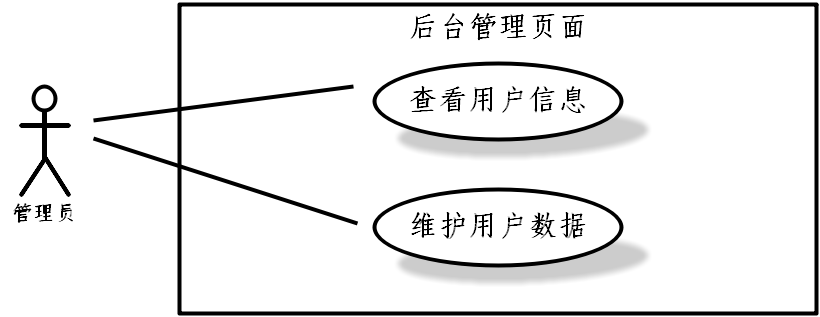
\includegraphics[scale=0.5]{image/f6.png}
	\caption{后台管理页面用例图}
\end{figure}

\begin{longtable}[c]{c|ccc}
	\caption{后台管理用例表}
	\label{tab:tab15}\\
	\shline
	\multicolumn{1}{c|}{\textbf{用例编号}} & \multicolumn{1}{c|}{UC-01} & \multicolumn{1}{c|}{用例名称} &  用户登录\\ \hline
	\endhead
	%
	\multicolumn{1}{c|}{\textbf{活动者}} & \multicolumn{1}{c|}{管理员} & \multicolumn{1}{c|}{优先级} &高  \\ \hline
	\textbf{用例描述} & \multicolumn{3}{p{12cm}}{该用例用来描述用户打开平台首页页面后,状态为未登录的用户通过输入账号和密码进行登录操作,系统将在登录过程中对用户账号及密码的正确性进行验证,并判断用户为个人用户还是企业用户,在登录后根据不同的账号类型在部分页面进行不同的页面显示。} \\ \hline
	\textbf{前置条件}& \multicolumn{3}{p{12cm}}{用户通过浏览器输入平台地址。} \\ \hline
	\textbf{基本事件流}& \multicolumn{3}{p{12cm}}{用户打开浏览器,在地址栏输入平台网址;\newline
		打开平台,展示平台首页;\newline
		用户账号为未登录状态,点击登录;\newline
		展示登录页面;\newline
		输入用户账号和密码进行验证。} \\ \hline
	\textbf{异常事件流}& \multicolumn{3}{p{12cm}}{1.网址URL 输入错误,打开平台首页失败;\newline
		2.用户账号或密码错误,登录失败。
	} \\ \hline
	\textbf{后置条件}& \multicolumn{3}{p{12cm}}{页面由登录页面回到首页,用户登录状态为已登录。} \\ \shline
\end{longtable}